\section{Erste Überlegungen test}

\begin{figure}
    \centering
    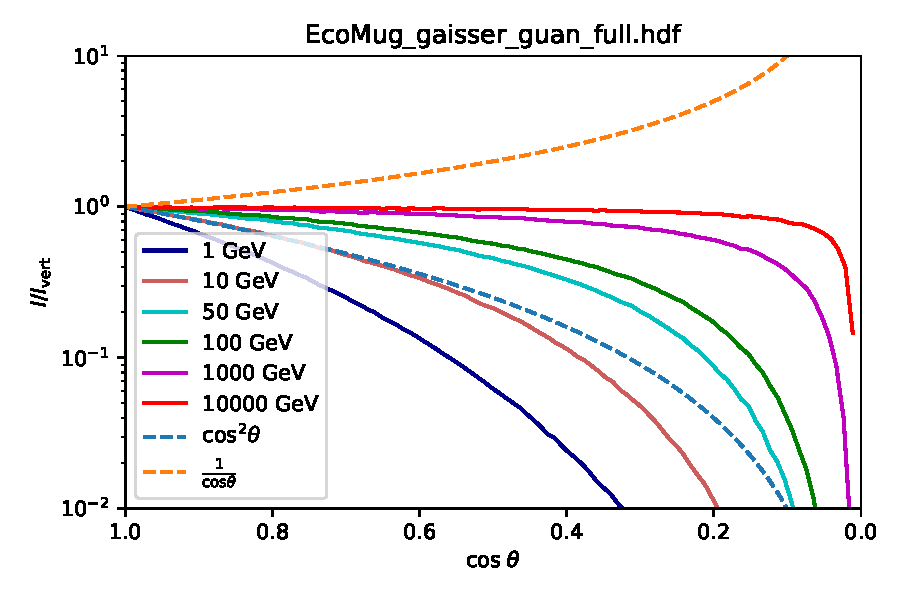
\includegraphics[width=8cm]{plots/plot.pdf}
    \caption{Zusammenhang }
    \label{fig:my_labels}
\end{figure}

Mein Ziel:

1. Untersuchen \textbf{wie} und  \textbf{in welchem Fall} man Myographie im Bergbau einsetzen kann.
\subsection{konkreter Anwendungsfall: Den Wasserstand ehemaliger Bergbaustollen überwachen.}

\textbf{Wie geht das ?}
Mit Detektor Myonen am Grund des "Beckens" dass mit Wasser vollläuft detektieren

\subsubsection{Zusammenhang Wassertiefe und Zählrate}

Auf der Erdoberflöche lässt sich eine Rate von

\begin{equation}
    1 \; \frac{\mathrm{muon}}{\mathrm{cm}^2 \; \mathrm{min}}
\end{equation} 

erwarten. Hiermit lässt sich einer Menge an simulierten Myonen eine echte 'Zeit' zuordnen die in der Wirklichkeit verstreichen müsste bis diese Menge aufgetreten ist.

Gemessen wird in einem Bohrloch mit einem Durchmesser von $10cm$.
Ein Zylinder-förmiger Detektor mit der Grundfläche von $75 cm^2$ bzw. $d=9,77cm$ ist realistisch.

An der Oberfläche lässt sich eine Detekor Rate von 
\begin{equation}
    108\; 000 \; \frac{\mathrm{N_\mathrm{\mu}}}{\mathrm{Tag}}
\end{equation}

annehmen.

Nun ergibt sich folgender \textbf{beispielhafter} Zusammenhang 
aus der Zählrate 
$counts \;per \;second$ und der Wasserhöhe $h$ im Bergbaustollen.

\begin{figure}[h]
    \centering
    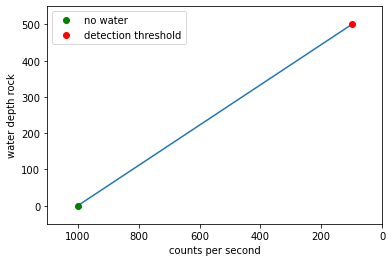
\includegraphics[width=8cm]{plots/rate_plot_example.png}
    \caption{Zusammenhang von Wassertiefe und Zählrate}
    \label{fig:my_label}
\end{figure}

Jetzt lässt sich aus einer gemessenen Zählrate eine Wassertiefe zuordnen.

\subsubsection{Statistische Grenzen}

Um eine sichere Aussage über die \textbf{'Stopping Power'} des Materials über dem Detektor zu bekommen, muss definiert werden bei \textbf{welcher Geometrie} des Detektors \textbf{wie lange} gemessen werden muss, um eine statistisch sichere Aussage treffen zu können.

Ein Ansatz um die minimale Zeit zu ermitteln die gemessen werden muss um statistisch sichere Myonen-Counts zu bekommen, wäre anschaulich immer die Zeit zu messen die verstreicht bis ein Myonen gemessen wird. 
Nun wird abgewartet bis die Standardabweichung aller Zeiten gering genug wird um den Präzision Ansprüchen zu genügen.

\begin{equation}
    \frac{t}{\text{event}}
\end{equation}
